\documentclass[12pt]{article}
\usepackage{a4}
\usepackage[english]{babel}
\setlength{\parindent}{0.35cm}
\pagestyle{headings}
\usepackage{graphicx}
\usepackage{grffile}
%Multiple picture in one figure
%\usepackage{subfigure}
\usepackage{subfig}
\usepackage[utf8]{inputenc}
\usepackage{listings}
\usepackage{color}
\usepackage{wrapfig}
%Floating-Umgebungen
\usepackage{float}
%Math-Environment
\usepackage{amsmath}
\usepackage{amssymb}
\usepackage{bbm}
%Better SI-Units
\usepackage{siunitx}
%Using Appendix
\usepackage[title]{appendix}
%Using URL
\usepackage[hidelinks]{hyperref}
%Using Colored Tables
\usepackage{colortbl}
\newcommand{\gray}{\rowcolor[gray]{.90}}
\usepackage{esvect}
% Use fancy tables
\usepackage{tabularx}
% Build fancy tables
\usepackage{booktabs}
% Configure enumeration
\usepackage{enumitem}
%Configure geometry
\usepackage{geometry}
\geometry{
	a4paper,
	left=3cm,
	right=3cm,
	top=3cm,
	bottom = 3cm,
	}

\lstset{
	language=C++,
	basicstyle=\small\ttfamily,
	keywordstyle=\color{blue}\ttfamily,
	stringstyle=\color{red}\ttfamily,
	commentstyle=\color{green}\ttfamily,
	morecomment=[l][\color{magenta}]{\#},
}


\usepackage{amsthm}

\renewcommand\qedsymbol{$\blacksquare$}
\newtheorem{theorem}{Theorem}[section]

\begin{document}
	
	\title{
		\textbf{\huge{CSE 446: Machine Learning Winter 2018 }} \\[2cm]
		\LARGE{Assignment 3 Bonus \\ \textcolor{red}{with bonus questions}}\\[1cm]
	}
	\author{from \\ Lukas Nies \\ University of Washington}
	\date{02/26/18}
	\clearpage\maketitle\thispagestyle{empty}
	\newpage

	\tableofcontents
	\setcounter{page}{0}
	\newpage
	
	% To start with section 1 labeled as section 0
	\setcounter{section}{-1}
	

\section{Policies}

\subsection{List of Collaborators}

My collaborator was Edith Heiter (discussed parts of Problem 1, 4, and 5 ). The development of the answers and code though was completely independent and individually.

\subsection{List of Acknowledgments}

None.

\subsection{Policies}

I have read and understood these policies.

\subsection{Note: Bonus included!}

In this version some of the bonus questions are included.

\newpage

\section{Problem: Linear Regression on MNIST}

\subsection{Closed Form Estimator}

\begin{enumerate}
	\item If one runs the Closed Form Estimator with $\lambda = 0$ one encounters trying to invert a singular matrix ($X^TX$) which is not possible per definition since the determinant is $\det(X^TX)=0$. The matrix is therefore not invertible. To avoid this we introduce a regularization by adding the term $\lambda\mathbbm{1}_d$. This is intuitively clear by considering the data itself: one digit consists of $28\times 28$ pixels where most pixels (at the edges and in the corners) don't carry any information about the digit itself (matrix is sparse). When calculating $X^TX$ we get the same result: we have more "dimensions" than information for those "dimensions". In mathematical terms: $X^TX$ is under-determined.
	\item For this part a grid search was implemented to search for different values of $\lambda$ and the threshold to optimize the performance on the development set:
		\begin{enumerate}[label=(\alph*)]
			\item The best result was found with $\lambda=0.02$ and a threshold of $0.5$. The grid search ran for $\lambda$ from 0.01 to 1 with steps of 0.01, the treshold ran from 0.1 to 1.0 in steps of 0.1.
			\item The average squared error using the parameters stated above is as follows:
				\begin{itemize}
					\item $\text{Training error}=0.013045$
					\item $\text{Development error}=0.01420$
					\item $\text{Test error}=0.01626$
				\end{itemize}
			\item The misclassification error using the parameters stated above is as follows:
			\begin{itemize}
				\item $\text{Training error}=0.93\%$
				\item $\text{Development error}=1.08\%$
				\item $\text{Test error}=1.76\%$
			\end{itemize}
		\end{enumerate}
	\item Samples with large values (far off the mean of the rest of the data points) have a strong influence on linear polynomial functions fitted through regression. This leads to large misclassification on most of the data points. A better model would be using a higher order polynomial to fit those samples more efficiently.
\end{enumerate}

\subsection{Linear regression using gradient descent}

\begin{enumerate}
	\item The proof is as follows:
		\begin{align*}
			\frac{\partial \mathcal{L}_\lambda}{\partial w} &= \frac{\partial}{\partial w} \left( \frac{1}{N} \sum_{n=1}^{N} \frac{1}{2} \left( y_n - w^Tx_n \right)^2 + \frac{\lambda}{2} \lVert w \rVert^2 \right) \\
			&= \frac{1}{N} \sum_{n=1}^{N} \left( -\frac{2x_n}{2} \right) \left( y_n - w^Tx_n \right) + \left( \frac{2\lambda}{2} \textbf{w}  \right) \\
			&= -\frac{1}{N} \sum_{n=1}^{N} \left( y_n - \hat{y}_n \right) x_n + \lambda \textbf{w}
		\end{align*}
	\item We can rewrite this as a matrix expression:
		\begin{align*}
			\frac{\partial \mathcal{L}_w}{\partial w} = -\frac{1}{N} \sum_{n=1}^{N} \left( y_n - \hat{y}_n \right) x_n + \lambda \textbf{w} = - \frac{1}{N} X^T \cdot \left( Y - \hat{Y} \right) + \lambda \textbf{w}
		\end{align*}
	\item Stepsizes $ -10^{-2} \leq \eta < -10^{-1} $ worked well for this problem. For the error rate see figure \ref{fig:1.2}. For generating the plots, $\eta = \frac{1}{4}\times 10^{-1}$ and $\lambda=10^{-2}$ were chosen.
		\begin{figure}[h!]
			\centering
			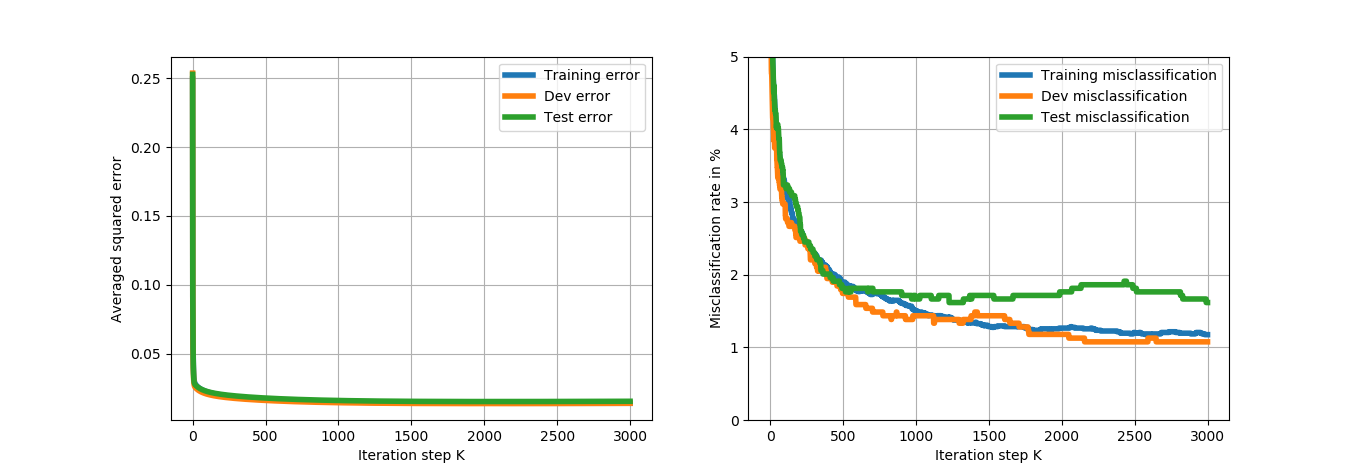
\includegraphics[width=\linewidth]{./Problem_1/Problem_1.2.png}
			\caption{Plot of averaged squared errors (left) and misclassification loss in percent (right) for the gradient descent algorithm. For generating the plots, $\eta = \frac{1}{4}\times 10^{-1}$ and $\eta=10^{-2}$ were chosen.}
			\label{fig:1.2}
		\end{figure}
	The lowest error I achieved is comparable to the closed form estimator, with $1.08\%$ on the development set. 
\end{enumerate}

\subsection{Linear Regression Using Stochastic Gradient Descent}

\begin{enumerate}
	\item The stochastic gradient descent diverges in this case with a learning rate for about $\eta=-0.1$ at $\lambda=0.005$. For too large values of $\eta$ the algorithm might never find the global minimum and therefore the gradient gets larger and larger which leads to divergence. 
	\item  Stepsizes $\eta \le -10^{-1} $ worked well for this problem. For the error rate see figure \ref{fig:1.3}. For generating the plots, constant $\eta = \frac{1}{4}\times 10^{-1}$ and $\eta=0.005$ were chosen.
	\begin{figure}[h!]
		\centering
		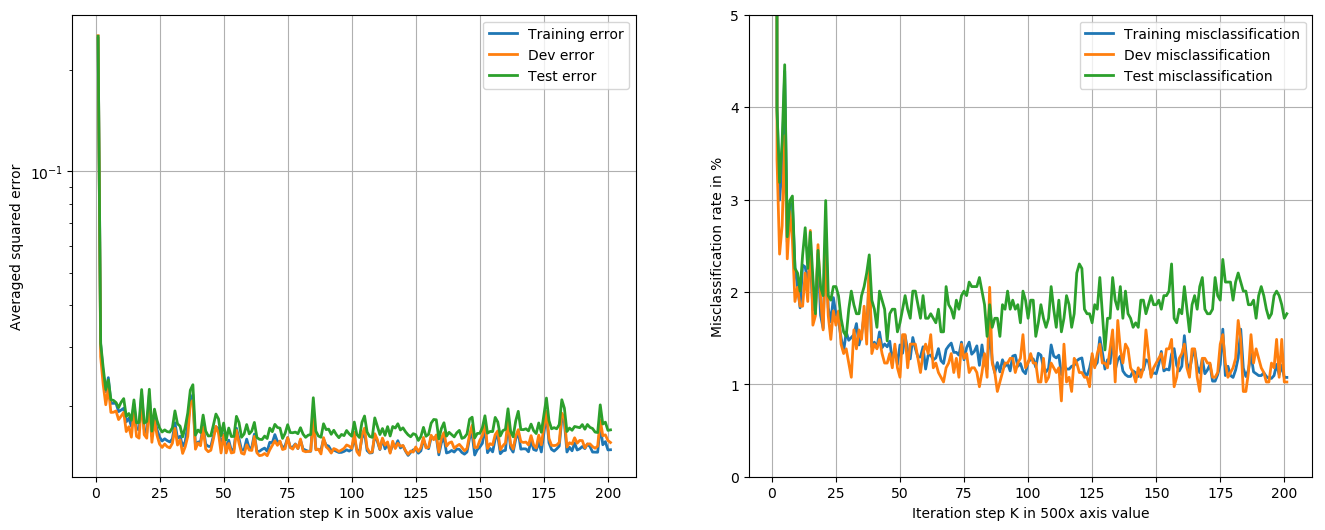
\includegraphics[width=0.85\linewidth]{./Problem_1/Problem_1.3.png}
		\caption{Plot of averaged squared errors (left, note the logarithmic vertical axis) and misclassification loss in percent (right) for the stochastic gradient descent algorithm. The horizontal axis shows the iteration steps for every 500th step. For generating the plots, $\eta = \frac{1}{4}\times 10^{-1}$ and $\eta=0.005$ were chosen.}
		\label{fig:1.3}
	\end{figure}
	The lowest error I achieved is comparable to the closed form estimator, with $1.03\%$ on the development set. 

\end{enumerate}

\subsection{\textcolor{red}{BONUS: Mini-batch stochastic gradient descent}}

\begin{enumerate}
	\item 
	\begin{enumerate}[label=(\alph*)]
		\item The stochastic gradient descent diverges in this case with a learning rate for about $\eta=-0.01$ at $\lambda=0.005$. This is ten times less than the stochastic gradient descent with $m=1$.
		\item Stepsizes $ -10^{-3} \leq \eta < -10^{-2} $ worked well for this problem. For the error rate see figure \ref{fig:1.4}. For generating the plots, $\eta = \frac{1}{4}\times 10^{-2}$ and $\lambda=0.005$ were chosen.
		\begin{figure}[h!]
			\centering
			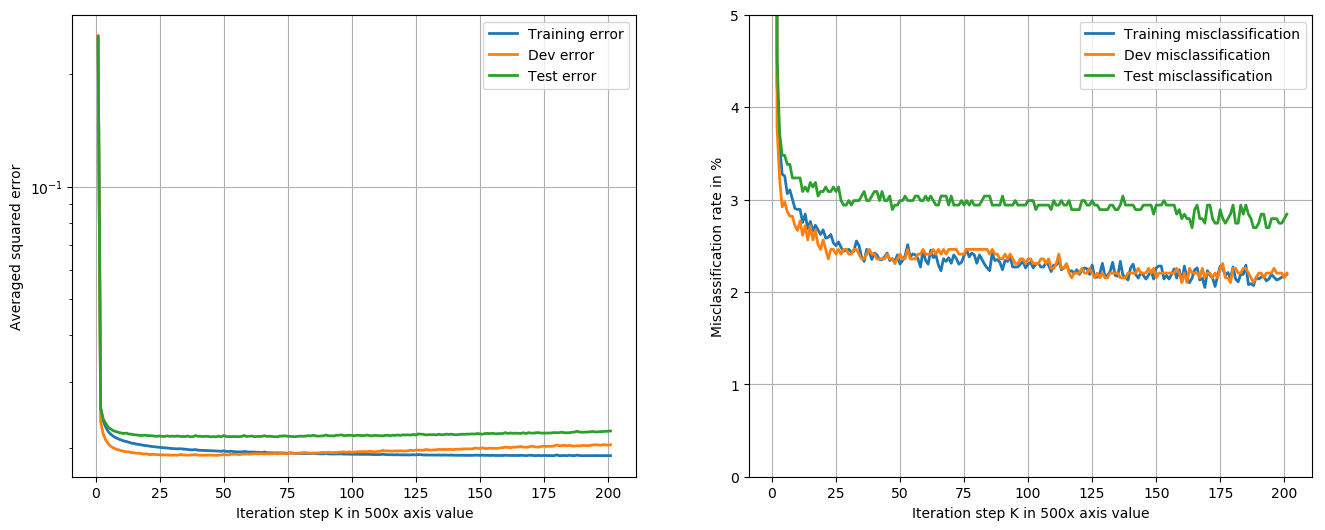
\includegraphics[width=0.85\linewidth]{./Problem_1/Problem_1.4.png}
			\caption{Plot of averaged squared errors (left, note the logarithmic vertical scale) and misclassification loss in percent (right) for the mini batch stochastic gradient descent algorithm with $m=100$. For generating the plots, $\eta = \frac{1}{4}\times 10^{-2}$ and $\lambda=0.005$ were chosen. The horizontal axis shows the iteration steps for every 500th step.}
			\label{fig:1.4}
		\end{figure}
		The lowest error I achieved was roughly $2.2\%$ on the development set.
	\end{enumerate}
	\item 
	By comparing plot \ref{fig:1.3} and \ref{fig:1.4} we find that the performance for the mini-batch algorithm is slightly worse than the normal stochastic gradient descent. The error rates increase by roughly $1\%$. In general the curves are more smooth since the gradient gets updated based on 100 random samples and not only on one random sample.
\end{enumerate}



\subsection{\textcolor{red}{BONUS: Using polynomial features}}

\begin{enumerate}
	\item We can calculate the dimensionality of the $\phi(x)$ vector by looking at at generic matrix $M$ of dimension $d$. The matrix consists of $d^2$ elements, where $d$ are diagonal elements and $d^2-d$ are non-diagonal elements. According to the problem, we need only the diagonal elements and half of the non-diagonal elements (to avoid counting pairs twice), so: 
	\begin{align}
		d_{\phi(x)} = \frac{d^2 - d}{2} + d = \frac{d^2+d}{2}
	\end{align}
	\item If we set $d=784$ then we would get $d_{\phi(x)}=307720$ features per sample. This isn't a good idea since the computation time for N=10000 samples with that amount of features would increase a lot because this results in roughly $10^9$ data points, respectively entries in the matrix. To work witch such a matrix with numpy arrays would fill the RAM with $8\times 10^9 = 8$GB of memory which probably throws an memory error. 
	\item For $d=40$ features we get $d_{\phi(x)}=820$ features per sample which yields in a massive reduction in computation time and use of memory. 
	\item Running with standard stochastic gradient descent, stepsizes $ -10^{-6} \leq \eta < -10^{-4} $ with $\lambda = 10^{-4}$ worked well for this problem. For the error rate see figure \ref{fig:1.5}. For generating the plots, $\eta = \times 10^{-5}$ and $\lambda=0.0001$ were chosen.
	\begin{figure}[h!]
	 	\centering
	 	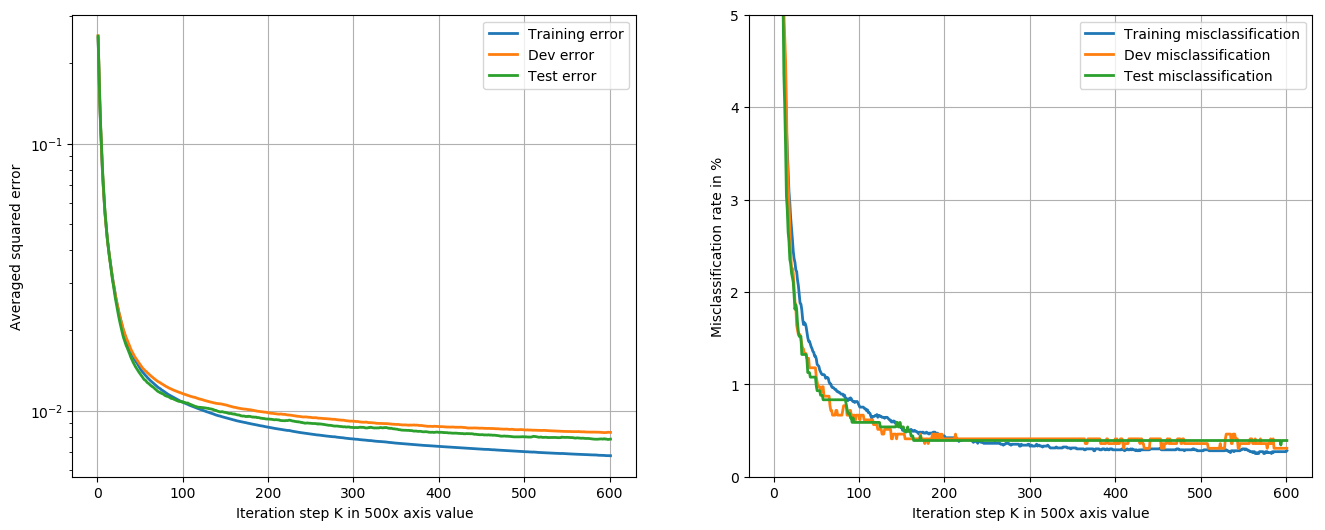
\includegraphics[width=0.85\linewidth]{./Problem_1/Problem_1.5.png}
	 	\caption{Plot of averaged squared errors (left, note the logarithmic vertical scale) and misclassification loss in percent (right) for the normal stochastic gradient descent algorithm with polynomial features. For generating the plots, $\eta = \times 10^{-5}$ and $\lambda=0.0001$ were chosen. The horizontal axis shows the iteration steps for every 500th step.}
	 	\label{fig:1.5}
	\end{figure}
	The lowest error I achieved was roughly $0.4\%$(!) on the development set.
\end{enumerate}


\newpage

\section{Binary Classification with Logistic Regression}

\begin{enumerate}
	\item For proofing this, we look at the cases $y_n=1$ and $y_n = 0$ separately.\\
	\noindent
	\underline{Case $y_n = 1$:}
	\begin{align*}
	\frac{\partial \mathcal{L}_\lambda}{\partial w} &= \frac{\partial}{\partial w} \left( -\frac{1}{N} \sum_{n=1}^{N} \log p_w (y_n = 1|x_n) + \frac{\lambda}{2}\lVert \textbf{w} \rVert^2  \right) \\
	&= \frac{\partial}{\partial w} \left( -\frac{1}{N} \sum_{n=1}^{N} \log\frac{1}{1+\exp(-wx_n)} + \frac{\lambda}{2}\lVert \textbf{w} \rVert^2  \right) \\
	&= \frac{\partial}{\partial w} \left( -\frac{1}{N} \sum_{n=1}^{N} \left[\log(1)-\log(1+\exp(-wx_n) \right] + \frac{\lambda}{2}\lVert \textbf{w} \rVert^2  \right) \\
	&= -\frac{1}{N} \sum_{n=1}^{N} \left[ \frac{x_n \exp(-wx_n)}{1+\exp(-wx_n)} \right] + \lambda\textbf{w}   \\
	&= -\frac{1}{N} \sum_{n=1}^{N} \left[ x_n(\hat{y}_n^{-1}-1)\hat{y}_n \right] + \lambda\textbf{w} = 
	-\frac{1}{N} \sum_{n=1}^{N} (1- \hat{y}_n)x_n + \lambda\textbf{w} 
	\end{align*}
	\underline{Case $y_n = 0$:}
	\begin{align*}
	\frac{\partial \mathcal{L}_\lambda}{\partial w} &= \frac{\partial}{\partial w} \left( -\frac{1}{N} \sum_{n=1}^{N} \log p_w (y_n = 0|x_n) + \frac{\lambda}{2}\lVert \textbf{w} \rVert^2  \right) \\
	&= \frac{\partial}{\partial w} \left( -\frac{1}{N} \sum_{n=1}^{N} \log\frac{1}{1+\exp(+wx_n)} + \frac{\lambda}{2}\lVert \textbf{w} \rVert^2  \right) \\
	&= \frac{\partial}{\partial w} \left( -\frac{1}{N} \sum_{n=1}^{N} \left[\log(1)-\log(1+\exp(+wx_n) \right] + \frac{\lambda}{2}\lVert \textbf{w} \rVert^2  \right) \\
	&= -\frac{1}{N} \sum_{n=1}^{N} \left[ \frac{-x_n \exp(+wx_n)}{1+\exp(+wx_n)} \right] + \lambda\textbf{w}   
	= -\frac{1}{N} \sum_{n=1}^{N} \left[ \frac{-x_n }{\exp(-wx_n)+1} \right] + \lambda\textbf{w}   \\
	&= -\frac{1}{N} \sum_{n=1}^{N}  -x_n\hat{y}_n + \lambda\textbf{w} = 
	-\frac{1}{N} \sum_{n=1}^{N} (0- \hat{y}_n)x_n + \lambda\textbf{w} 
	\end{align*}
	\item We can rewrite this as a matrix expression:
	\begin{align*}
	\frac{\partial \mathcal{L}_\lambda}{\partial w} = -\frac{1}{N} \sum_{n=1}^{N} \left( y_n - \hat{y}_n \right) x_n + \lambda \textbf{w} = - \frac{1}{N} X^T \cdot \left( Y - \hat{Y} \right) + \lambda \textbf{w}
	\end{align*} 
	\item Properties of logistic regression
	\begin{enumerate}[label=(\alph*)]
		\item Suppose the data is linear separable and $\lambda=0$. In order to fit the data best, one would like to optimize the sigmoid function $\frac{1}{1+\exp(-wx)}$. Since the data is linear separable all, data points with $y_n=0$ are left of $x=0$ and all points with $y_n=1$ are to the right. In this case, the optimal fit would be the Heaviside function (step function, 0 for $x<0$, 1 for $x>0$). In order to optimize the sigmoid function to approach the Heaviside function, $w\rightarrow \inf$. Hence, our weight vector would diverge. 
		\item If we suppose that $d>n$ ($\lambda=0$) then the data matrix is sparse and several features will carry no information (equal 0). To fit a larger accumulation of features with value 0 the logistic function must approach, similar to previous question, the Heaviside function. Therefore the weight vector will diverge.
		\item To avoid the divergence of the weight vector one can introduce regularization which avoids sparsity and linear separability such that the algorithm stops early enough to give a good estimation without diverging too fast. If one does not consider this the algorithm might overfit which influences the true error.
	\end{enumerate}
						
\end{enumerate}

\subsection{\textcolor{red}{BONUS: Log loss, applied}}

\begin{enumerate}
	\item 
	For tackling this problem I chose a batch size of $m=100$, a step size of $\eta=\frac{1}{4}\times 10^{-2}$ and a parameterization factor of $\lambda=0.01$.
	\begin{figure}[h]
		\centering
		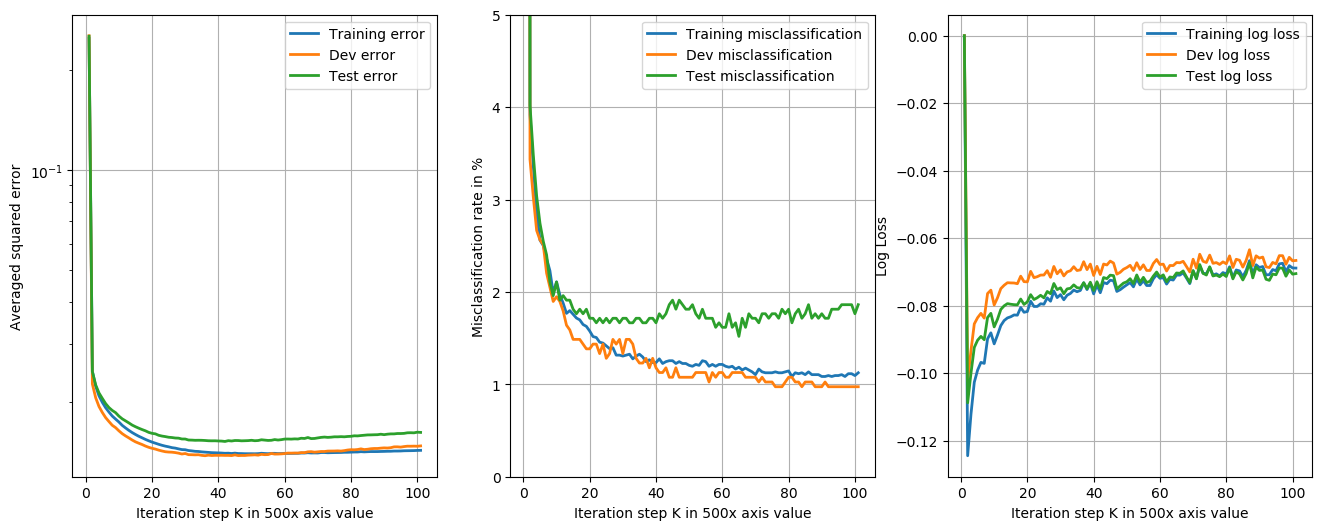
\includegraphics[width=1\linewidth]{./Problem_2/Problem_2.1_normal_features.png}
		\caption{Plot of averaged squared errors (left, note the logarithmic vertical scale), the misclassification loss in percent (middle) and the log loss (right) for the mini batch stochastic gradient descent algorithm with normal features. For generating the plots, $\eta = \times \frac{1}{4}\times 10^{-2}$ and $\lambda=0.01$ were chosen. The horizontal axis shows the iteration steps for every 500th step.}
		\label{fig:2.1}
	\end{figure}
	\item 
	Again, I chose a batch size of $m=100$, a step size of $\eta=\frac{1}{4}\times 10^{-2}$ and a parameterization factor of $\lambda=0.01$.
	\begin{figure}[h]
		\centering
		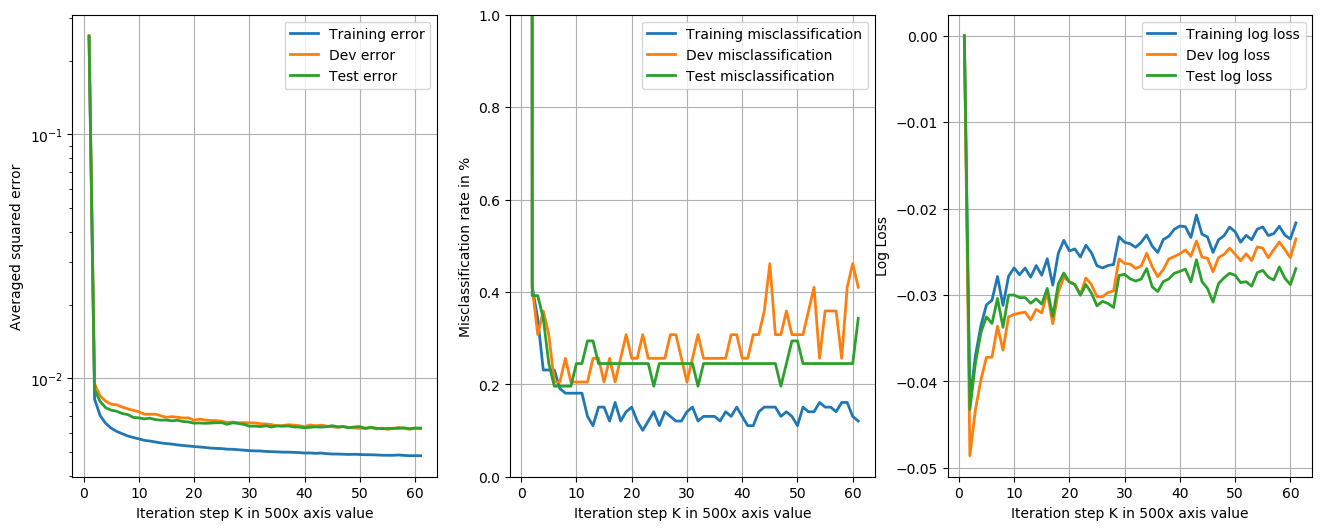
\includegraphics[width=1\linewidth]{./Problem_2/Problem_2.1_pol_features.png}
		\caption{Plot of averaged squared errors (left, note the logarithmic vertical scale), the misclassification loss in percent (middle) and the log loss (right) for the mini batch stochastic gradient descent algorithm with normal features. For generating the plots, $\eta = \times \frac{1}{4}\times 10^{-2}$ and $\lambda=0.01$ were chosen. The horizontal axis shows the iteration steps for every 500th step.}
		\label{fig:2.2}
	\end{figure}
\end{enumerate}

\newpage\phantom{blabla}
\newpage\phantom{blabla}

\section{Multi-Class classification using Least Squares}

\subsection{"One vs. all Classification" with Linear Regression}

\begin{enumerate}
	\item We can rewrite this as a matrix expression:
	\begin{align*}
	\frac{\partial \mathcal{L}_W}{\partial W} = -\frac{1}{N} \sum_{n=1}^{N} x_n\left(  y_n - \hat{y}_n \right)^T + \lambda \textbf{W} = - \frac{1}{N} X^T \cdot \left( Y - \hat{Y} \right) + \lambda \textbf{W}
	\end{align*}
	\item Stepsizes $ -10^{-2} \leq \eta \le -10^{-1} $ worked well for this problem using the stochastic gradient descent. For the error rate see figure \ref{fig:3.1}. For generating the plots, $\eta = \frac{2}{4}\times 10^{-1}$ and $\eta=10^{-2}$ were chosen.
	\begin{figure}[h!]
		\centering
		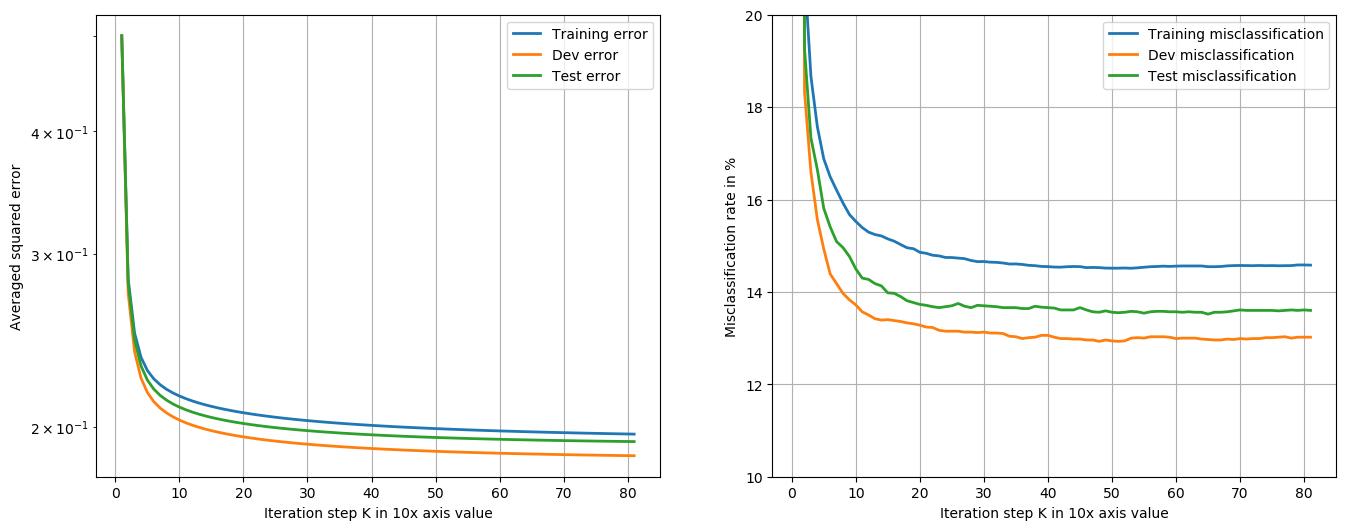
\includegraphics[width=\linewidth]{./Problem_3/Problem_3.1.png}
		\caption{Plot of averaged squared errors (left) and misclassification loss in percent (right) for the gradient descent algorithm. For generating the plots, $\eta = \frac{1}{4}\times 10^{-1}$ and $\eta=10^{-2}$ were chosen.}
		\label{fig:3.1}
	\end{figure}
	The lowest error I achieved is roughly 13\% on the development set.
\end{enumerate}

\subsection{\textcolor{red}{BONUS: Matrix derivative}}

Following the matrix derivative:
\begin{align}
	\mathcal{L}_W &= \notag \frac{1}{2N}\sum_{n=1}^{N}\lVert y_n -W^Tx_n\rVert_2^2+\frac{\lambda}{2}\lVert W \rVert_2^2=\frac{1}{2N}\lVert Y-X\cdot W\rVert_2^2 + \frac{\lambda}{2}\lVert W \rVert_2^2 \\ \notag
	&= \frac{1}{2N}\left[ (Y - X\cdot w)^T(Y-X\cdot w) \right] + \frac{\lambda}{2}W^TW\\
	\frac{\partial \mathcal{L}_W}{\partial W} \notag &= \frac{1}{2N}\left[ -2X^T (Y-X\cdot W) + \lambda W \right] = -\frac{1}{N}X^T(Y-X\cdot W) + \lambda W \\
	&= -\frac{1}{N}\sum_{n=1}^{N} x_n(y_n - \hat{y}_n)^T + \lambda W
\end{align}

\subsection{\textcolor{red}{BONUS: Softmax}}

Calculate the derivative according to previous problem parts as a general case of the one hot encoding with $k$ possible different label and the softmax probability distribution. Therefore:
\begin{align}
	\frac{\partial \mathcal{L}_W}{\partial W} = -\frac{1}{N}\sum_{n=1}^{N}x_n(y_n-\hat{y}_n)^T + \lambda W = - \frac{1}{N} X^T (Y-\hat{Y}) + \lambda W
\end{align}
\noindent
The dimensions are 
\begin{align*}
	X\in \mathbb{R}^{n\times d} && Y \in \mathbb{R}^{n\times k} && \hat{Y}\in\mathbb{R}^{n\times k} && W \in \mathbb{R}^{d\times k}
\end{align*}
For our dataset $k=10$.



\newpage

\section{Probability and Maximum Likelihood Estimation}

\subsection{Probability Review}

\begin{enumerate}
	\item 
	\begin{enumerate}[label=(\alph*)]
		\item Since the disease is quite rare it is likely that one does not have the disease even if one is tested positive. The amount of healthy persons in a group is larger than the number of sick persons and even if the test is highly accurate it's much more likely that one is healthy given the test is incorrect. 
		\item The probability of being tested positive (P) given having the disease ($\bar{H}$) is given by:
		\begin{align}
			P(P|\bar{H})=\frac{P(\bar{H}|P)P(P)}{P(\bar{H})}=0.99.
		\end{align}
		By reversing this Bayesian theorem we can yield the probability having the disease given being tested positive:
		\begin{align}
			P(P|\bar{H})=\frac{P(\bar{H}|P)P(\bar{H})}{P(P)},
		\end{align}
		where $P(P)$ is the total probability being tested positive, which is the sum of the probabilities of being tested positive and being sick, or being tested positive and being healthy:
		\begin{align}
		P(\bar{H}|P)&=\frac{P(P|\bar{H})P(\bar{H})}{P(P)}=\frac{P(P|\bar{H})P(\bar{H})}{P(P|\bar{H})P(\bar{H})+P(P|H)P(H)}\\
		&=\frac{0.99\times 10^{-4}}{0.99\times 10^{-4}+0.01\times(1-10^{-4})}=\frac{1}{102}=0.98\%
		\end{align}
	\end{enumerate}
	\item We can rewrite the table as follows:
	% Table generated by Excel2LaTeX from sheet 'Sheet1'
	\begin{table}[h!]
		\centering
		\begin{tabular}{|c|c|c|c|}
			\toprule
			& S=0   & S=1   &  \\
			\midrule
			C=1   & P(S=0 $\cap$ C=1)    & P(S=1 $\cap$ C=1)    & P(C=1) \\
			\midrule
			C=0   & P(S=0 $\cap$ C=0)    & P(S=1 $\cap$ C=0)    & P(C=0) \\
			\midrule
			& P(S=0) & P(S=1) & 1 \\
			\bottomrule
		\end{tabular}%
	\end{table}% 
	\begin{table}[h!]
		\centering
		\begin{tabular}{|c|c|c|c|}
			\toprule
			& S=0   & S=1   &  \\
			\midrule
			C=1   & $\frac{23}{151}$    & $\frac{34}{151}$    & $\frac{57}{151}$  \\
			\midrule
			C=0   & $\frac{41}{151}$    & $\frac{53}{151}$    & $\frac{94}{151}$  \\
			\midrule
			& $\frac{64}{151}$  & $\frac{87}{151}$  & 1 \\
			\bottomrule
		\end{tabular}%
	\end{table}%
	It follows:
	\begin{enumerate}[label=(\alph*)]
		\item $\hat{p}(C=1,S=1)=P(C=1\cap S=1)=\frac{34}{151}=22.52\%$
		\item $\hat{p}(C=1|S=1)=\frac{P(C=1\cap S=1)}{P(S=1)}=\frac{34}{87}=39.08\%$
		\item $\hat{p}(C=0|S=0)=\frac{P(C=0\cap S=0)}{P(S=0)}=\frac{41}{64}=64.06\%$
	\end{enumerate}
	\item A hat over a parameter denotes an estimator of the parameter. The estimator estimates a probability value of an event based on a limited amount of samples whereas the actual probability of an event is given by looking at all samples.    
\end{enumerate}

\subsection{Maximum Likelihood Estimation}

\begin{enumerate}
	\item If the observations are independent then the likelihood function is given by the product of the probability mass function which is the Poisson distribution in this case:
	\begin{align}
		l(\lambda, G_1,\dots, G_N)=\prod_{i=1}^{N}\frac{\lambda^{G_i}}{G_i!}\exp(-\lambda)
	\end{align}
	Therefore the log-likelihood function is given applying the (natural) logarithm:
	\begin{align}
		L(\lambda, G_1,\dots, G_N)&= \ln\left( \prod_{i=1}^{N}\frac{\lambda^{G_i}}{G_i!}\exp(-\lambda)  \right)= \sum_{i=1}^{N}\left[ \ln\left( \frac{\lambda^{G_i}}{G_i!}\exp(-\lambda) \right) \right] \notag \\
		&= \sum_{i=1}^{N}\left[  \ln(\lambda^{G_i})-\ln(G_i!)+\ln(\exp(-\lambda)) \right] \notag \\
		&= \sum_{i=1}^{N}\left[  G_i\ln(\lambda)-\ln(G_i!)-\lambda\right]
	\end{align}
	\item In order to find the MLE for $\lambda$ we need to solve
	\begin{align}
		\hat{\lambda}=\arg\max_\lambda(L(\lambda, G_1,\dots, G_N))
	\end{align}
	by taking the derivative in respect to $\lambda$:
	\begin{align}
		\frac{\partial}{\partial\lambda}\left( L(\lambda, G_1,\dots, G_N) \right) &= 0. \\ \notag
		\Leftrightarrow
		0 &= \frac{\partial}{\partial\lambda}\left(\sum_{i=1}^{N}\left[  G_i\ln(\lambda)-\ln(G_i!)-\lambda\right]  \right) \notag \\
		\Leftrightarrow
		0 &= \sum_{i=1}^{N}\left[  \frac{G_i}{\hat{\lambda}}-1\right] = -N + \frac{1}{\lambda}\sum_{i=1}^{N}G_i \notag \\
		\Leftrightarrow
		\hat{\lambda} &= \frac{1}{N}\sum_{i=1}^{N}G_i. 
	\end{align}
	\item The MLE for $\lambda$ using the observed G is therefore:
	\begin{align}
		\hat{\lambda} &= \frac{1}{N}\sum_{i=1}^{N}G_i. = \frac{1}{8}\left( 6+4+2+7+5+1+2+5 \right) = 4
	\end{align}
	
\end{enumerate}

\section{BONUS: State of the art on MNIST}

Disclaimer: As stated bt the instructor in the problem set we do not have a dev set. To create a small dev set I chopped of 30 data points from the test set to roughly tune my hyperparameters on this small dev set. This size is chosen to lie within the $3\sigma=99.7\%$ confidence interval to guaranty a good estimation of the test error even by looking a little bit on the test set. As it appears after finishing this problem, this was a good choice to estimate the squared average error but not the misclassification rate.  \par 
A word to bias: after failing by adding bias before mapping the features I added bias after mapping as one data point in the mini batch sample. This leads to some improvement in the overall results. 

\subsection{\textcolor{red}{BONUS: Start small ($k=5000$)}}

\begin{enumerate}
	\item I am aware that for different choices of $\lambda$ the algorithm diverges sooner or later. For very small $\lambda$ one can choose higher step sizes without diverging too early, for larger $\lambda$ one must use smaller step size to avoid diverging. For $\eta=0.0001$ and $\lambda=0.01$ I found good results. The learning rate was constant. For this given $\lambda$ the algorithm diverges for $\eta=10^{-2}$.
	\item See figure \ref{fig:5.1}.
	\begin{figure}[b]
		\centering
		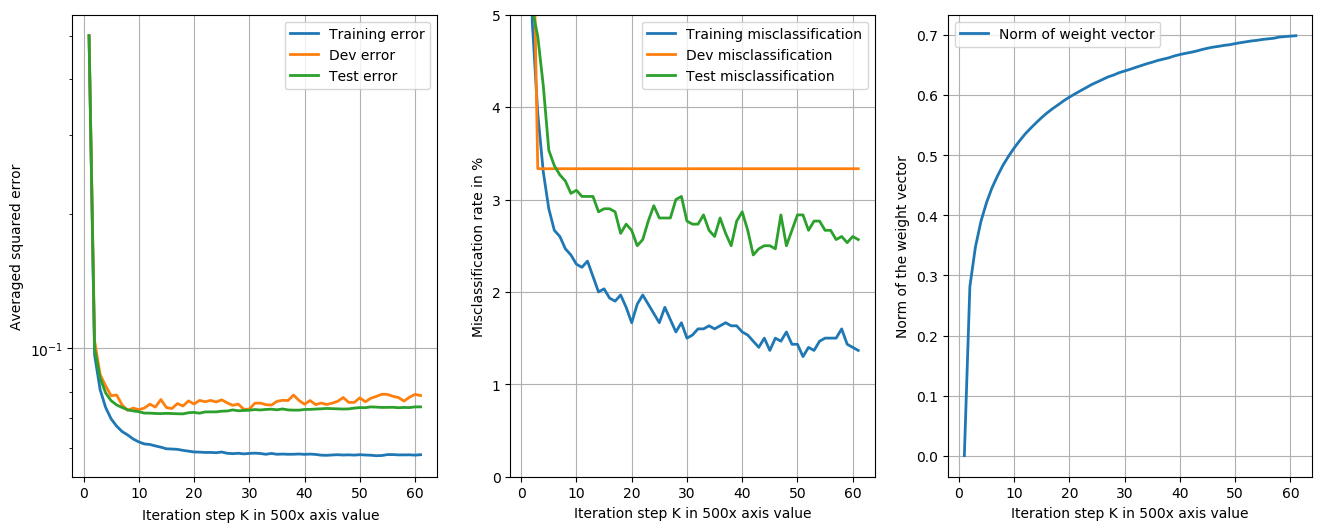
\includegraphics[width=\linewidth]{./Problem_5/Problem_5.1.png}
		\caption{Case $k=5000$. Plot of averaged squared errors (left), the norm of the weight vector (right) and misclassification loss in percent (middle). For generating the plots, $\eta = 10^{-3}$ and $\lambda=10^{-2}$ were chosen.}
		\label{fig:5.1}
	\end{figure}
	\item See figure \ref{fig:5.1}.
	\item See figure \ref{fig:5.1}. Comment: The norm of the weight vector appears to look like a root function or logarithm function. Since neither of those two function families converges for large iterations I can not make an assumption about convergence of the norm. But to me it looks like for large iterations the norm might be upper bounded by one.  
	\item 
	\begin{itemize}
		\item Lowest training avg. sq. error: 0.05756
		\item Lowest test avg. sq. error: 0.07140
	\end{itemize}
	\item
	\begin{itemize}
		\item Lowest training miscl. error: 1.30\%
		\item Smallest \# of total mistakes for training set: 780/60000
		\item Lowest test miscl. error: 2.40\%
		\item Smallest \# of total mistakes for test set: 239/10000
	\end{itemize}
	\underline{Comment on overfitting}: It clearly can be seen that the misclassification error for the training set and test set separate for early iteration steps (around step 500 to 1000). For late iterations, both error rates roughly converge with a difference of about 1\%. \\
	\noindent
	\underline{Comment on choice of dev set:} As stated before, the (tiny) dev set gives a good estimation for the squared error but is a little off for estimating the misclassification rate. Though it gave some intuition about the order of magnitude of the errors.
\end{enumerate}

\subsection{\textcolor{red}{BONUS: Go big ($k=60000$)}}

For evaluating the errors in this part I chose a subset of 3000 random data points in test and training set. The dev set was chosen like the one in previous part.

\begin{enumerate}
	\item For $\lambda=0.01$ and $\eta=10^{-3}$ I found good results. The learning rate was constant. For this given $\lambda$ the algorithm diverges for $\eta=10^{-2}$.
	\item See figure \ref{fig:5.2}.
	\begin{figure}[b]
		\centering
		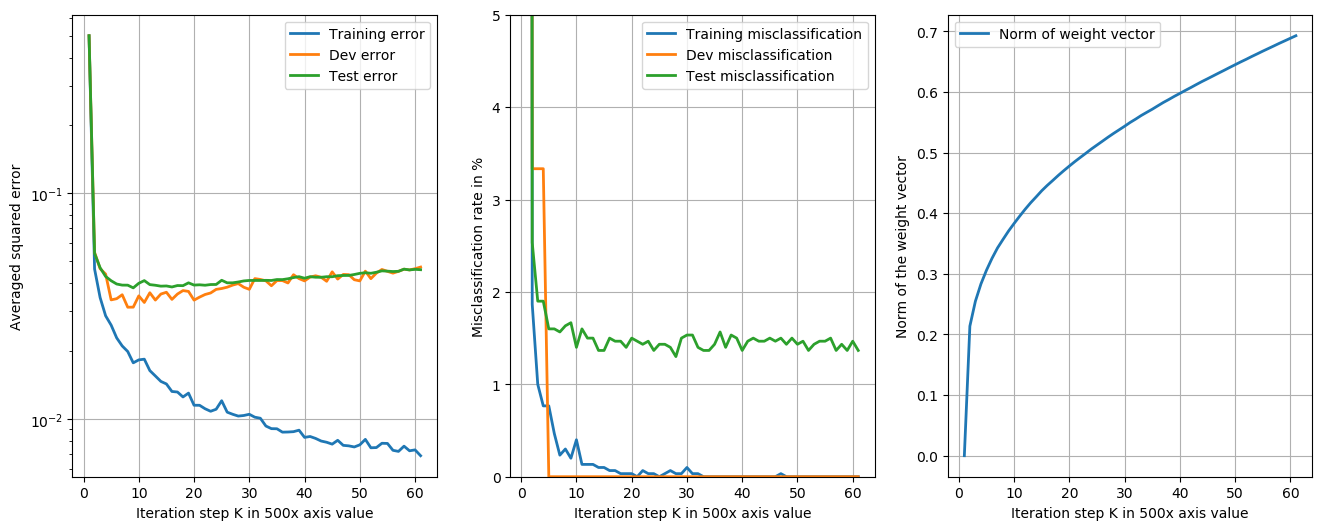
\includegraphics[width=\linewidth]{./Problem_5/Problem_5.2.png}
		\caption{Case $k=60000$. Plot of averaged squared errors (left), the norm of the weight vector (right) and misclassification loss in percent (middle). For generating the plots, $\eta = 10^{-3}$ and $\lambda=10^{-2}$ were chosen.}
		\label{fig:5.2}
	\end{figure}
	\item See figure \ref{fig:5.2}.
	\item See figure \ref{fig:5.2}. Comment: Again one can find a root like or logarithmic like behavior but compared to the smaller feature size the slope for later iterations is steeper. 
	\item 
	In order to get good run times and to prevent running out of memory, the errors were calculated on a 3k subset.
	\begin{itemize}
		\item Lowest training avg. sq. error: 0.00687
		\item Lowest dev avg. sq. error: 0.03129
		\item Lowest test avg. sq. error: 0.03812
	\end{itemize}
	\item
	In order to get good run times and to prevent running out of memory, the errors were calculated on a 3k subset.
	\begin{itemize}
		\item Lowest training miscl. error: 0.00\%
		\item Smallest \# of total mistakes for training set: 0/60000
		\item Lowest dev miscl. error: 0.00\%
		\item Smallest \# of total mistakes for dev set: 0/30
		\item Lowest test miscl. error: 1.30\%
		\item Smallest \# of total mistakes for test set: 129/10000
	\end{itemize}
	\item
	\underline{Comment on overfitting}: In the case for using all the features we can clearly see the curse of overfitting. While the training error literally goes to zero for later iterations, the test error separates after around 500 to 1000 iteration steps and converges to roughly 1.4\%. The trained algorithm does no mistakes on the training set but still does about 130 mistakes out of 10000 predictions. Now looking at the average squared error one can see that the test error has a minimum around 2500 iterations and then slowly rises again whereas the training error still falls. To avoid overfitting and to get a good error estimation one should consider stopping training early, around the first 5000 iterations. \\
	\noindent
	\underline{Comment on choice of dev set:} See previous part.
\end{enumerate}



%\chapter*{Bibliography}
\addcontentsline{toc}{chapter}{Bibliography}%	


\bibliographystyle{unsrt}
\bibliography{./bib}
/


\end{document}  